\subsection{Gæsteoprettelse}
\label{sub:GuestCreator}

Gæsteoprettelsesmodulet har til opgave at oprette en ny gæst i databasen.

\subsubsection{Funktionalitet}
\label{ssub:GuestCreator_funktionalitet}

Gæsteoprettelsesmodulet tilgås fra loginmodulet, når der ønskes, at oprette en ny gæst. Gæsten indtaster dernæst information omkring sig selv, båden samt udrejse dato. Gæsten gemmes til slut i databasen, hvis den indtastede information er tilfredsstillende.

\begin{figure}
  \centering
  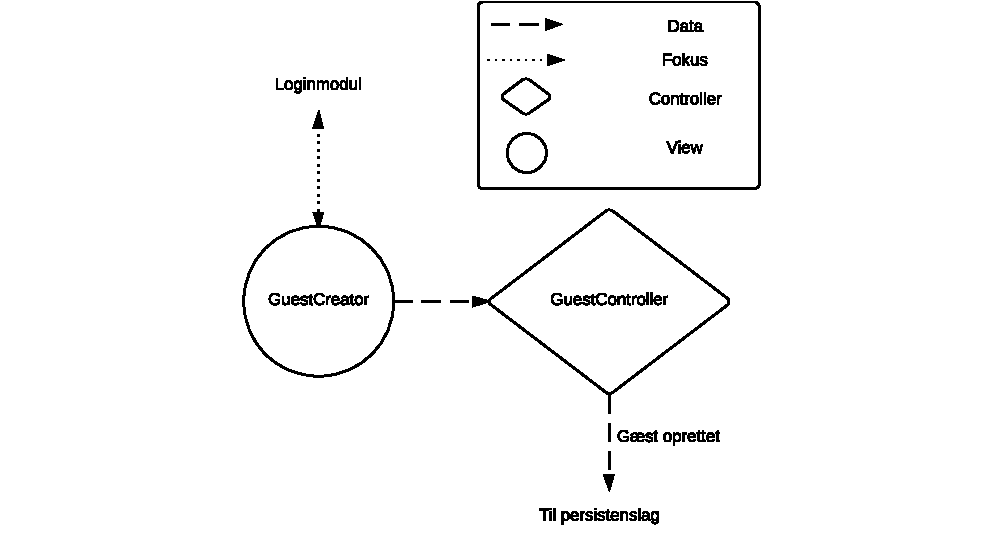
\includegraphics[width=\textwidth]{newguest-diagram.pdf}
  \caption{Diagram over gæsteoprettelsesmodulet}
  \label{fig:guestcreator}
\end{figure}

\subsubsection{Implementation}
\label{ssub:GuestCreator_implementation}

Gæsteoprettelsesmodulet, der fremstår som \enquote{Ny Gæst} på \cref{fig:guestcreator}, består af et GuestCreator-view og en GuestController. Den data der indtastes i GuestCreator view'et, sendes videre til GuestControlleren. Herefter kommunikerer GuestControlleren med persistenslaget, som derefter gemmer informationen om den nye gæst.
